\documentclass[conference]{IEEEtran}
\IEEEoverridecommandlockouts


% The preceding line is only needed to identify funding in the first footnote. If that is unneeded, please comment it out.
\usepackage{cite}
\usepackage{amsmath,amssymb,amsfonts}
\usepackage{algorithmic}
\usepackage{graphicx}
\usepackage{textcomp}
\usepackage{xcolor}
\usepackage{array}
\usepackage{booktabs}
% Custom column type (centered with fixed width)
\newcolumntype{C}[1]{>{\centering\arraybackslash}p{#1}}

\def\BibTeX{{\rm B\kern-.05em{\sc i\kern-.025em b}\kern-.08em
    T\kern-.1667em\lower.7ex\hbox{E}\kern-.125emX}}
\renewcommand\IEEEkeywordsname{Keywords}
\begin{document}

\title{Evaluating Cardiovascular Disease Risk Through PCA-Driven Machine Learning Models.
}

\author{\IEEEauthorblockN{1\textsuperscript{st} Abu Nayeem}
\IEEEauthorblockA{\textit{Department of Computer Science} \\
\textit{American International University-Bangladesh (AIUB) }\\
Dhaka, Bangladesh \\
21-45933-3@student.aiub.edu}
\and
\IEEEauthorblockN{2\textsuperscript{nd} Hasibur Rahman }
\IEEEauthorblockA{\textit{Department of Computer Science} \\
\textit{American International University-Bangladesh (AIUB) }\\
Dhaka, Bangladesh \\
21-45676-3@student.aiub.edu}
\and
\IEEEauthorblockN{3\textsuperscript{rd} Mamun Sarkar}
\IEEEauthorblockA{\textit{Department of Computer Science} \\
\textit{American International University-Bangladesh (AIUB) }\\
Dhaka, Bangladesh \\
22-46170-1@student.aiub.edu}
\and
\IEEEauthorblockN{4\textsuperscript{th} Dipongkor Roy}
\IEEEauthorblockA{\textit{Department of Computer Science} \\
\textit{American International University-Bangladesh (AIUB) }\\
Dhaka, Bangladesh \\
21-45490-3@student.aiub.edu}
\and

}


\maketitle

\begin{abstract}
Cardiovascular disease (CVD) remains the leading cause of mortality globally, highlighting the urgent need for effective early detection systems. Supervised machine learning algorithms, such as Logistic Regression (LR), SGDClassifier (SDGC), Support Vector Classifier (SVC), K-Nearest Neighbors (KNN), Decision Tree (DT), Random Forest (RF), Gradient Boosting (GB), AdaBoost (AB), LightGBM (LGBM), and XG- Boost (XGB), are applied to the Framingham Heart Study (FHS) data set to predict mortality risk and are presented in this research in a comparative analysis. In the proposed study, Principal Component Analysis (PCA) is applied to reduce the number of dimensions of the model and increase its usability and effectiveness. The performance measures in the model were accuracy, precision, recall, F1 score, and AUC-ROC. The stability of the model was checked with the help of 10-fold cross validation. Furthermore, the results of the study show that ensemble models outperform linear and intermediate accuracy classifiers but in respect of predictive accuracy and generalization. In RF and XGB, the test accuracy was 98.05\% and the F1 score was 0.98 and 98.04\% correspondingly, and the robustness was also similar, and the precision recall balance was greater. Moreover, it has been established that PCA is useful in minimizing the model complexity as well as significantly hence retaining a large amount of variance. These findings support the notion that the combination of ensemble learning and dimensionality reduction methods with wearable-compatible, real-time cardiovascular monitoring devices can help scale and provide an intervention with high accuracy to individuals who are at risk.
\end{abstract}

\vspace{1em}

\begin{IEEEkeywords}
Cardiovascular Risk Prediction, Dimensionality Reduction, Ensemble Learning, Machine Learning, Supervised Classification, Wearable Health Monitoring.
\end{IEEEkeywords}

\section{Introduction}
Cardiovascular diseases (CVDs) stand as the main global cause of mortality since they generate yearly mortality rates of 17.9 million deaths which represent 32\% of total global deaths [1]. Most of the deaths associated with CVD may be avoided through symptom testing and treatment services during the initial stages of disease progression particularly in locations that experience poor access to healthcare.  The present healthcare setting allows implementing the principles of machine learning (ML) and artificial intelligence (AI) to create new risk evaluation systems that can reveal at-risk individuals before the severe cases of medical emergencies appear [2].  The increasing health data in wearable technology and clinical documentation. provides artificial intelligence models an opportunity to establish scalable and customized monitoring to continue early risk assessment on the basis of analysis.  Machine learning (ML) and deep learning algorithms have become a major trend in the contemporary healthcare field and assist in the detection of illnesses at a young stage in cases of diabetes, cancer, and cardiovascular illnesses [3].

\vspace{1em}

ML algorithms can identify non-linear and complicated patterns in large multidimensional data that are not otherwise identified by traditional statistical techniques. Due to the long-term nature of this information, which also includes such vital risk factors as age, blood pressure, cholesterol, smoking status, and glucose levels, the FHS dataset is often used in studies on cardiovascular disorders [4]. The ML models utilize these medical datasets to develop prediction systems that can provide a decision support and an automated alert. Ensemble methods such as RF, GB, and eXtreme Gradient Boosting (XGBoost) work well since they are able to deal with both linear and non-linear characteristics without overfitting [5]. The dimensionality reduction plays an important role in enhancing speed and generalization, especially in case of dealing with noisy data provided by wearable measure devices. This is often done using PCA, and in this case it helps to improve the model by removing redundancy at a cost of the least important data variance. This combination of ensemble learning and dimensionality reduction enhances the model’s efficiency in real-time health monitoring systems.



\vspace{1em}

Ensemble classifiers were tested on the Framingham data with high results to predict risk of ten-year coronary heart disease [6]. They define such risk factors as blood pressure, glucose, and tobacco use as important and work with unbalanced data effectively. Previous studies do not have a consistent evaluation of linear, non-linear and ensemble models using PCA-transformed features, however. The gap is bridged in this work through the testing of ten supervised models: LR, SGDClassifier, SVC, KNN, DT, RF, GB, AB, LGBM and XGB. Some of the metrics include accuracy, precision, recall, F1 score, AUC-ROC, and 10-fold cross-validation [7]. RF and XGB are superior in the field of precision and generalization. To ensure the early detection of the wearable or mobile machine learning system, the proposed architecture integrates effective classification and dimensionality reduction.
 


\section{Related Work}
They have attracted the attention of numerous researchers [8] who used them to predict cardiovascular disease through the means of Machine Learning or Artificial Intelligence and various datasets like EHR, a wearable sensor stream or a clinician diagnostic. Though these studies showcase substantial progress in risk assessment and early detection, most uses of the studies are biased, their scope is limited by the fact that they focus on a model or a dataset, and the combination of the reduction of dimensions, model interpretation, and cross-model review is rare.

\vspace{1em}

Zhang et al. [8] proposed an ML pipeline to predict CVD with the help of wearable sensor data, and electronic health records (EHRs). They found that to improve the early CVD detection, RF and LR were capable of real time processing of wearable data. However, their exploration did not provide an extensive comparison of algorithms and discussed very few models. Krittanawong et al. [9] used deep learning on clinical and imaging data to predict cardiac risk. They highlighted the fact that convolutional neural networks (CNNs) can detect cardiac problems well, however, they also mentioned that they are opaque regarding clinical judgments. This further motivated the necessity to have more interpretable models, including tree-based ensembles, in the healthcare industry. Shameer et al. [10] identified three significant barriers to AI technology in their assessment of how it could be utilized in cardiovascular care: issues in the implementation of wearable systems, disparity in data, and lack of interpretability. They suggested that robust classifiers in conjunction with dimension-reduction could enhance accuracy and make the model more applicable in scarce resource environments. Ensemble methods like AB and XGB are superior to simple models, when combined with proper preprocessing, which is feature selection and normalization, as reported by Alizadehsani et al. [11]. They, however, indicated that a regular pipeline and feature engineering are important to the output.

\vspace{1em}

Dey et al. [12] compared some of the supervised learning methods on Cleveland and Statlog heart disease datasets. Even though their results spoke in favor of the use of RF and KNN in the healthcare domain, they did not pay much attention to dimensionality reduction and advanced boosting methods, which too affected generalization. Ensemble and interpretable models have gained popularity in predicting heart disease in the context of wearable health, especially in recent years. Although Kumar et al. [13] conducted a combination of PCA and explanatory algorithms such as XGB to minimize the computer load and enable the real-time detection of a CVD at a relatively low amount of information loss, they also performed a combination of LGBM and SHAP values to obtain high accuracy and the clarity of decisions to make in a wearable-based monitoring system. A combination of these studies indicates that there has been an increasing use of robust ensembles along with dimensionality reduction to develop interpretable and generalizable predictive systems. Nonetheless, very limited literature has been able to provide a consistent study of the effectiveness of linear and ensemble classifiers on wearable data that are converted by means of PCA. This paper seeks to bridge that gap by providing a comparative, in-depth analysis, which is suitable in cardiovascular risk assessment in the real world.



\section{METHODOLOGY}
\subsection{Dataset Description}
The research utilized cardiovascular risk data available on Kaggle with 4240 instances which contained 16 features that included age, gender and various other demographic, behav- ioral and physiological measurements. The database contained ’ten year chd’ as the target variable which indicated coronary heart disease development during a ten-year observation period (value 1 represented ’Yes’ and value 0 showed ’No’). The workflow diagram of the proposed system is shown in Fig. 1.

\begin{figure}[h!]
    \centering
    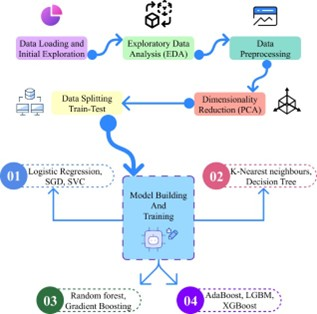
\includegraphics[width=0.45\textwidth]{Picture1.jpg}
    \caption{Workflow Diagram of the Proposed System}
    \label{fig:myphoto}
\end{figure}


\subsection{Data Preprocessing}\label{AA}
\begin{itemize}
\item \textbf{Exploratory Data Analysis (EDA):} Basic statistics, distributions, and correlation matrices were analyzed to understand feature relationships.
\item \textbf{Handling Class Imbalance:} The distribution of the target variable was imbalanced. Techniques such as oversam- pling and class-weight adjustments were considered [14].
\item \textbf{Feature Scaling and Encoding:} Continuous features were normalized using Min-Max scaling, and categorical variables were label encoded.
\item \textbf{Dimensionality Reduction:} PCA was applied to reduce feature dimensions while preserving maximum variance. Mathematically, PCA projects the data $\mathbf{X}$ onto a lower- dimensional space using the eigenvectors of the covariance matrix
$\mathbf{\Sigma}$:

\vspace{1em}

\begin{equation}
\text{PCA}(\mathbf{X}) = \mathbf{X}\mathbf{W} \label{eq:pca}
\end{equation}
\end{itemize}

where, $\mathbf{W}$ represents the eigenvectors corresponding to the largest eigenvalues of $\Sigma$.

\subsection{\textbf{Model Selection and Mathematical Formulation}}

Multiple classification models were implemented and evaluated:

\subsubsection{\textbf{Logistic Regression (LR)}}
A linear model that estimates the probability $p$ of the binary class using the logistic function:

\begin{equation}
p(y=1 \mid \mathbf{x}) = \frac{1}{1 + e^{-(\mathbf{w}^T \mathbf{x} + b)}}
\end{equation}

where $\mathbf{w}$ and $b$ are the weight vector and bias term.

\subsubsection{\textbf{Stochastic Gradient Descent (SGD)}}
SGD minimizes the logistic loss function via gradient updates:

\begin{equation}
\mathcal{L}(\mathbf{w}) = \sum_{i=1}^{n} \log(1 + e^{-y_i (\mathbf{w}^T \mathbf{x}_i)})
\end{equation}

The weights are updated as:

\begin{equation}
\mathbf{w}_{t+1} = \mathbf{w}_t - \eta \nabla \mathcal{L}(\mathbf{w}_t)
\end{equation}

where $\eta$ is the learning rate.

\subsubsection{\textbf{Support Vector Classifier (SVC)}}
SVC constructs a hyperplane that maximizes the margin between two classes:

\begin{equation}
\min_{\mathbf{w}, b} \frac{1}{2} \|\mathbf{w}\|^2 \quad \text{subject to} \quad y_i (\mathbf{w}^T \mathbf{x}_i + b) \geq 1
\end{equation}

where $y_i \in \{+1, -1\}$.

\subsubsection{\textbf{K-Nearest Neighbors (KNN)}}
KNN classifies a sample based on the majority label among its $k$ nearest neighbors, using Euclidean distance:

\begin{equation}
d(\mathbf{x}_i, \mathbf{x}_j) = \sqrt{\sum_{k=1}^{n} (x_{ik} - x_{jk})^2}
\end{equation}

\subsubsection{\textbf{Decision Tree Classifier (DT)}}
DT split the feature space to reduce impurity, using Gini impurity:

\begin{equation}
\text{Gini}(D) = 1 - \sum_{i=1}^{C} p_i^2
\end{equation}

where $p_i$ is the proportion of samples belonging to class $i$.

\subsubsection{\textbf{Random Forest Classifier (RF)}}
RF is an ensemble of DT built on bootstrapped data with random feature selection. The final prediction is obtained via majority voting:

\begin{equation}
\hat{y} = \text{mode}\left(\{h_t(\mathbf{x})\}_{t=1}^{T}\right)
\end{equation}

where $h_t(\mathbf{x})$ is the prediction of the $t$-th tree.

\subsubsection{\textbf{Gradient Boosting Classifier (GB)}}
GB builds models sequentially by optimizing a differentiable loss function, typically the logistic loss for classification:

\begin{equation}
F_m(\mathbf{x}) = F_{m-1}(\mathbf{x}) + \gamma_m h_m(\mathbf{x})
\end{equation}

where $\gamma_m$ is the step size and $h_m(\mathbf{x})$ is the $m$-th weak learner.

\subsubsection{\textbf{AdaBoost Classifier (AB)}}
AB updates instance weights based on misclassifications in each iteration. The weight of the $m$-th weak learner is computed as:

\begin{equation}
\alpha_m = \frac{1}{2} \ln\left(\frac{1 - \varepsilon_m}{\varepsilon_m}\right)
\end{equation}

where $\varepsilon_m$ is the classification error of the $m$-th weak learner.

\subsubsection{\textbf{LightGBM Classifier (LGBM)}}
LGBM grows trees in a leaf-wise (best-first) manner rather than level-wise, allowing faster convergence. It optimizes a regularized objective function:

\begin{equation}
\mathcal{L}(\theta) = \sum_{i=1}^{n} l(y_i, f(x_i)) + \Omega(f)
\end{equation}

where $l(y_i, f(x_i))$ is the loss function and $\Omega(f)$ is the regularization term controlling model complexity.

\subsubsection{\textbf{XGBoost Classifier (XGB)}}
XGB extends GB with additional regularization to reduce overfitting. The objective function is defined as:

\begin{equation}
\mathcal{L}(F) = \sum_{i=1}^{n} l(y_i, F(x_i)) + \Omega(f_k)
\end{equation}

with:

\begin{equation}
\Omega(f_k) = \gamma T + \frac{1}{2} \lambda \|\mathbf{w}\|^2
\end{equation}

where $T$ is the number of leaves in the tree and $\lambda$ controls the L2 regularization on leaf weights.






\subsection{\textbf{Model Evaluation Metrics}}

The performance of each model was evaluated using the following metrics:

\begin{itemize}
    \item \textbf{Accuracy:}
    \begin{equation}
    \text{Accuracy} = \frac{TP + TN}{TP + TN + FP + FN}
    \end{equation}
    
    \item \textbf{Precision:}
    \begin{equation}
    \text{Precision} = \frac{TP}{TP + FP}
    \end{equation}
    
    \item \textbf{Recall (Sensitivity):}
    \begin{equation}
    \text{Recall} = \frac{TP}{TP + FN}
    \end{equation}
    
    \item \textbf{F1 Score:}
    \begin{equation}
    \text{F1 Score} = 2 \times \frac{\text{Precision} \times \text{Recall}}{\text{Precision} + \text{Recall}}
    \end{equation}
    
    \item \textbf{ROC AUC:} Measures the model's ability to distinguish between classes across various thresholds. AUC closer to 1 indicates superior classification performance.
\end{itemize}

\subsection{\textbf{Cross-Validation Strategy}}

To ensure robustness and reduce overfitting, 10-fold cross-validation was applied. The data were split into ten parts, with each part used once for testing and nine times for training, and the final score is the average across all folds \cite{s4}. To improve interpretability, we applied SHAP (SHapley Additive exPlanations) to the RF and XGB models. SHAP highlighted age, systolic blood pressure, and glucose as the top features, findings that match known CVD risk factors and add transparency to the used models.

\section{Results And Discussion}

This section presents and analyzes the performance of various supervised learning models on the FHS dataset. The models were evaluated using standard metrics like accuracy, precision, recall, F1 score, and ROC AUC, along with visual tools such as confusion matrices, correlation heatmaps, and cross-validation charts to assess their effectiveness and generalization.

\subsection{\textbf{Performance Comparison: Accuracy Across Models}}

\begin{figure}[h]
\centerline{
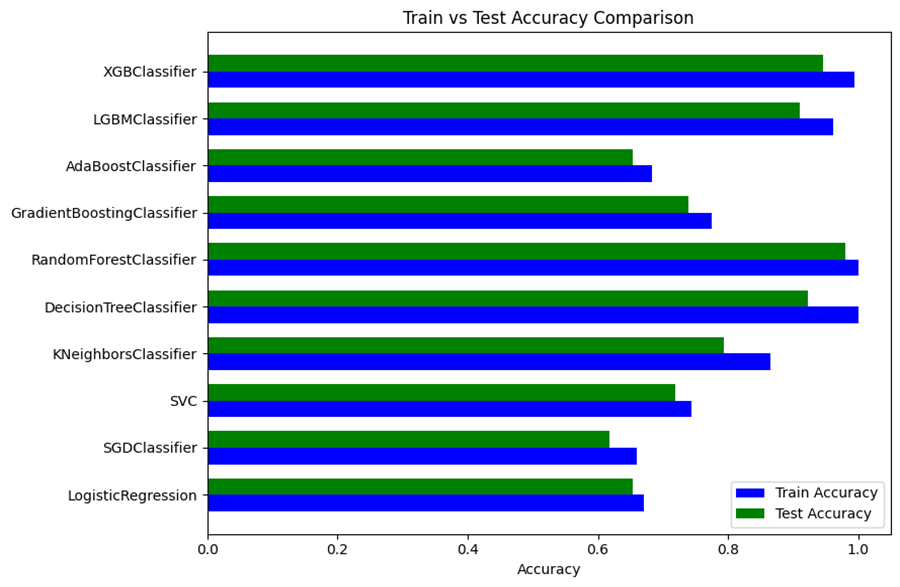
\includegraphics[width=0.5 \textwidth]{Picture2.png}}
\caption{Training vs Testing Accuracy Comparison}
\label{fig:1}
\end{figure}

Fig.\ref{fig:1} compares the testing and training accuracy of ten ML models. XGB has the highest accuracy of training, and the lowest testing dip, which explains the best performance.  LGBM also generalizes excellently and is also good at its performance.  The test accuracy of AB is significantly lower, which means that it is likely to be either overfitting or that it is a sensitive test.  GB maintains a good balance of testing and training.  Both DT and RF achieved 100\% training accuracy, however, only RF generalized well, which was test accuracy of 98.05\% compared to 82.36\% of DT.  This means that in DT, there is overfitting that was reduced in RF using ensemble, cross-validation and PCA.  The patterns of test data could have been the reason why KNN had a slightly higher test accuracy than training.  LR and SGDC were the worst whereas SVC was fixed in both sets. Overall, the chart shows which models are generalized and can be applied in the real world.



\begin{table*}[t]
\centering
\caption{Performance Comparison of Machine Learning Models on PCA-Transformed Framingham Data}
\label{tab:model_performance}
\renewcommand{\arraystretch}{1.3}
\begin{tabular}{C{3cm} C{2cm} C{2.2cm} C{2.2cm} C{1.29cm} C{1.29cm} C{1.29cm}}
\toprule
\textbf{Model} & \textbf{Best PCA Components} & \textbf{Train Accuracy} & \textbf{Test Accuracy} & \textbf{Precision} & \textbf{Recall} & \textbf{F1 Score} \\
\midrule
LR     & 11 & 0.6713 & 0.6539 & 0.6403 & 0.6676 & 0.6537 \\
SGDC          & 13 & 0.6597 & 0.6185 & 0.6135 & 0.5952 & 0.6042 \\
SVC                     & 14 & 0.7434 & 0.7192 & 0.6948 & 0.7599 & 0.7259 \\
KNN     & 3  & 0.8651 & 0.7929 & 0.7261 & 0.9261 & 0.8140 \\
DT           & 1  & 1.0000 & 0.9222 & 0.8663 & 0.9943 & 0.9259 \\
RF          & 14 & 1.0000 & 0.9805 & 0.9681 & 0.9929 & 0.9804 \\
GB       & 15 & 0.7746 & 0.7394 & 0.7123 & 0.7841 & 0.7465 \\
AB                & 15 & 0.6833 & 0.6532 & 0.6368 & 0.6776 & 0.6566 \\
LGBM                & 14 & 0.9619 & 0.9097 & 0.8670 & 0.9631 & 0.9125 \\
XGB                 & 13 & 0.9937 & 0.9465 & 0.9087 & 0.9901 & 0.9477 \\
\bottomrule
\end{tabular}
\end{table*}

\subsection{\textbf{Performance Comparison: F1 Score Evaluation}}



Fig. \ref{fig:2} compares the accuracy and recall of every model against each other by comparing the F1 scores. XGB and RF perform the best with almost similar ratings of about 1.0. LGBM also has good generalization. GB and DT are also reliable but a little weaker. SGDC and LR have dismal F1 scores of approximately 0.6, whereas AB, KNN, and SVC is plausible. In medical usage, the comparison can be used to find out the models that maintain a balanced quality of prediction that is vital in dealing with false positives and false negatives.

\begin{figure}[h]
\centerline{
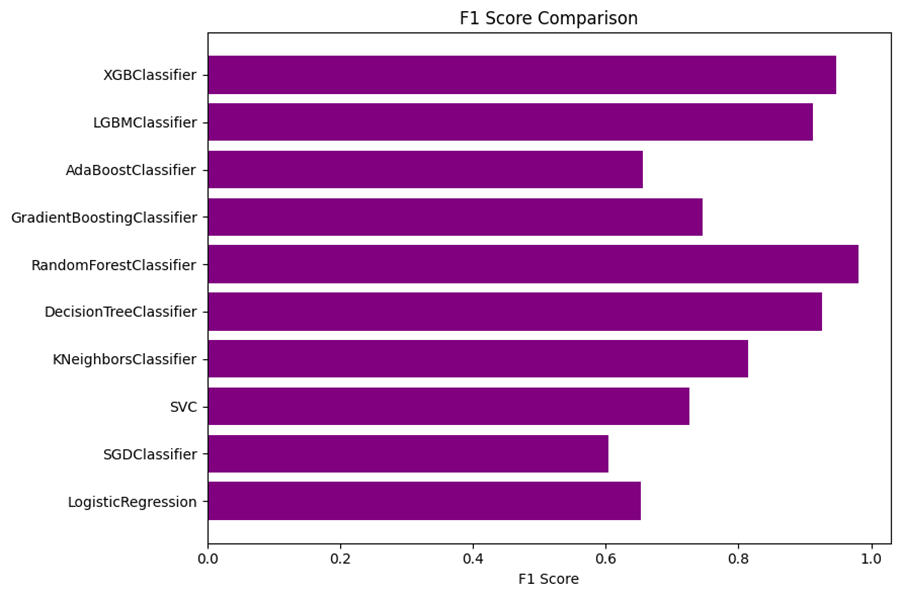
\includegraphics[width=0.5 \textwidth]{Picture3.png}}
\caption{F1 Score Comparison Across Different Models}
\label{fig:2}
\end{figure}

\subsection{\textbf{Confusion Matrix Analysis}}


\begin{figure}[h]
\centerline{
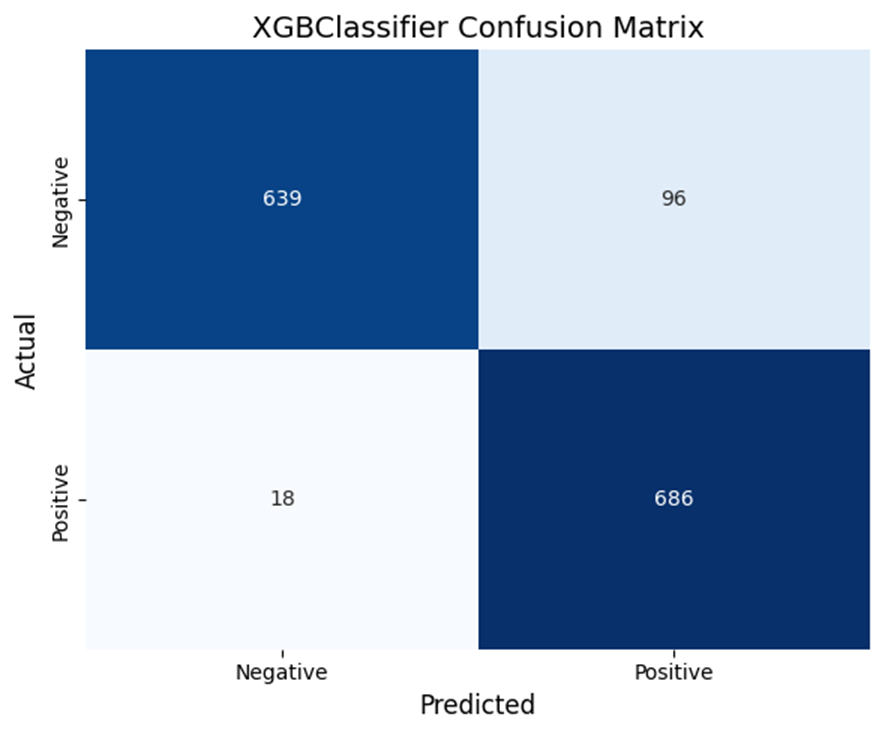
\includegraphics[height=6cm, width=0.5 \textwidth]{Picture4.png}}
\caption{The confusion matrix of the XGBoost classifier}
\label{fig:3}
\end{figure}



Fig. \ref{fig:3} provides an in-depth evaluation of the performance of the XGB classifier predictions. The values in the matrix are the real values as compared to the best values per the negative class, 639 true negatives and 96 false positives are expected in the negative class which means that the model has failed to identify some of the negative cases correctly, however, it has done well in the positive cases. Knowledge of false positives helps to enhance the effects of wearable characteristics such as blood pressure, heart rate, or glucose to create accurate predictions, but false negatives ensure that at-risk people are not overlooked. Based on this confusion matrix, it is possible to state that the model is performing well, with very few misclassifications.



\begin{figure}[h]
\centerline{
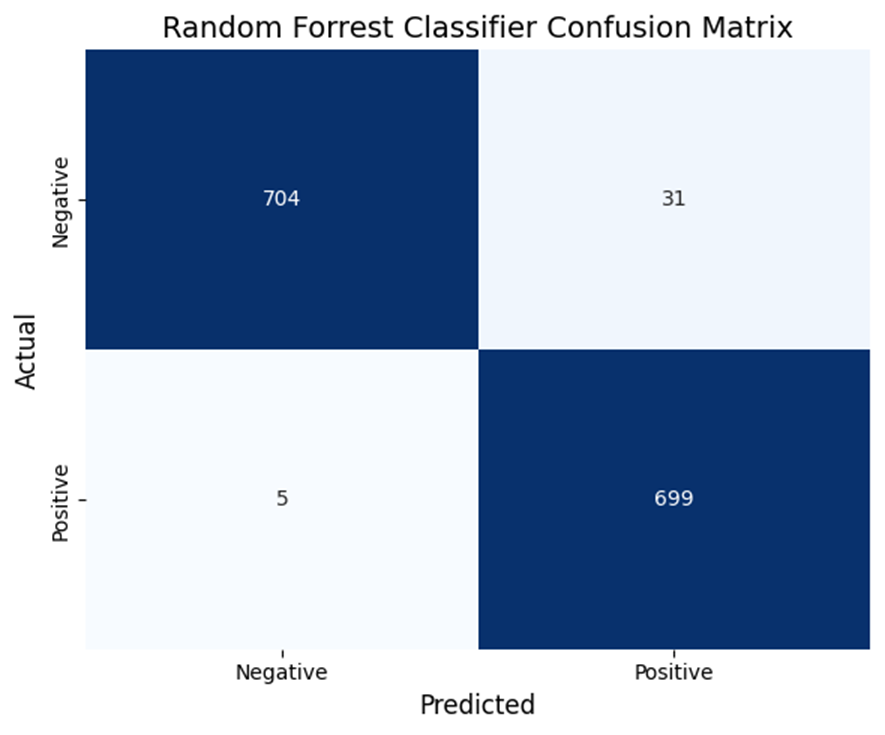
\includegraphics[height=6cm,width=0.5 \textwidth]{Picture5.png}}
\caption{Confusion Matrix of the Random Forest Classifier}
\label{fig:4}
\end{figure}

The confusion matrix of the RF Classifier is presented in Fig. \ref{fig:4} on the test set. The model only identified 31 false positives and 5 false negatives and rightly identified 704 negative and 699 cases. This high sensitivity-specificity ratio portrays the reliability of this model. These error rates are so low, and this is essential to mortality prediction because the wrong identification of a high-risk person can be fatal. The results indicate that the RF model is suitable to medical risk evaluation based on wearable device data because it manages to differentiate between at-risk and healthy individuals.


\subsection{\textbf{ROC-AUC Curve Comparison}}

\begin{figure}[h]
\centerline{
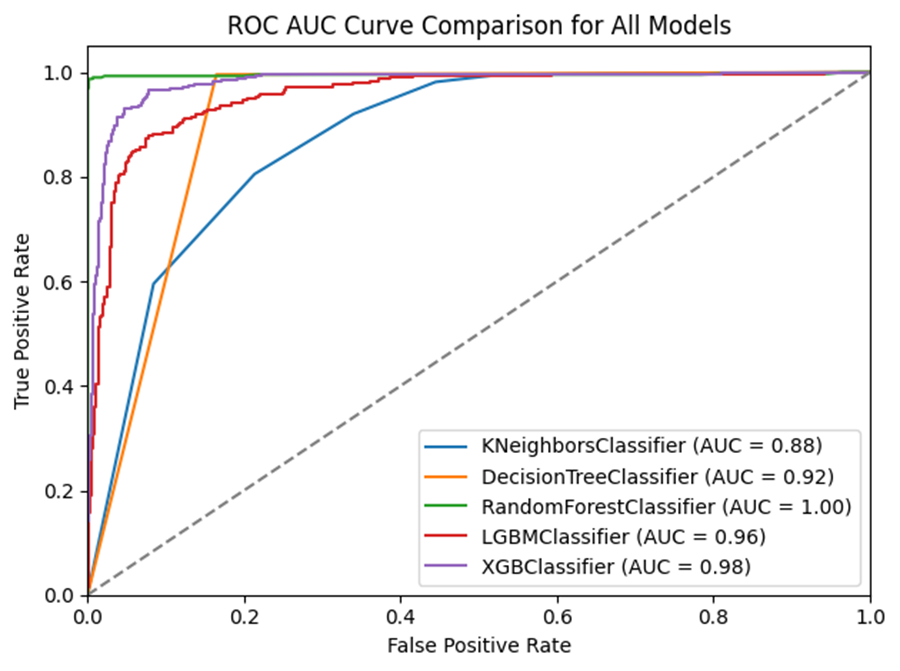
\includegraphics[width=0.5 \textwidth]{Picture6.png}}
\caption{ROC \& AUC Curve Comparison }
\label{fig:6}
\end{figure}

Fig. \ref{fig:6} shows the ROC AUC curves for different models, providing a comparison of their classification performance. The diagonal dashed line depicts a random classifier that does not have predictive power, and better model performance is represented by the curves above the diagonal dashed line. Having excellent classification potential, the RF Classifier and XGB Classifier are rated 1.0 and 0.98 respectively in the AUC ratings. The other models like the DT Classifier and the KNN Classifier have lower AUCs, which suggest that they have a lower degree of predictive power. The early intervention is determined by the capability of the model to be able to continually distinguish between the high-risk and the low-risk individuals, indicated by a large AUC. Graphics are a handy tool that can be used to understand the ability of different models to differentiate between the positive classes and the negative ones.


\subsection{\textbf{Cross-Validation Stability of Ensemble Models}}


Fig. \ref{fig:7} compares the 10-fold cross-validation of the RF and XGB models. Every point represents the accuracy of a fold. RF has more steady results, whereas XGB is more uneven, especially in the first ones. Overall, the two models are quite precise, but RF is more stable. This helps in determining the stability of the models and is the way the models would perform when using new untested patient data. Healthcare environments that require wearable-embedded models to be able to deliver credible and generic predictions are required because of the diversity of the situations and circumstances of the individuals.



\begin{figure}[h]
\centerline{
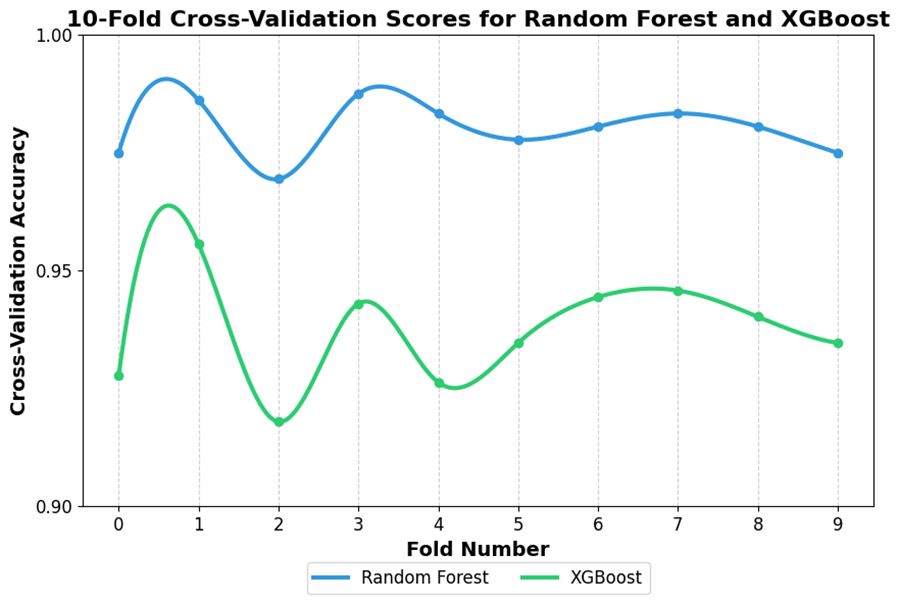
\includegraphics[width=0.5 \textwidth]{Picture7.png}}
\caption{10-Fold Cross validation for Random Forest and XGBoost}
\label{fig:7}
\end{figure}


Table \ref{tab:model_performance} summarizes how different ML models performed in predicting mortality using PCA-transformed Framingham data. Each model was adjusted to contain the most desirable number of principal components. RF was the highest in test accuracy (98.05\%) and F1 score (0.980) with an excellent accuracy and recall. XGB also showed good performance with a score of F1= 0.948 and an accuracy of 94.65\%, able to handle complex patterns comfortably. LGBM has a high recall (0.963) and F1 score (0.913), so it can be used in those scenarios when it is essential to avoid instances of missing. KNN can result in the generation of more false positives due to low precision (0.726) and excellent recall (0.926). Linear models (LR and SGDC) had poor test accuracy of less than 66\%.  Both RF and DT had perfect training accuracy but only RF could maintain high test performance, but overfitting was observed in DT.  Everything said and done, the ensemble models like RF, XGB and LGBM gave the best results and are more applicable in predicting risks of CVD using wearables in the real world.

\section{Conclusion}
The CVD risk prediction using PCA transformed features from FHS dataset was evaluated with ten supervised machine learning models in this research. The ensemble-based models such as the RF, XGB, and LGBM performed better in the cross validation based on the accuracy, precision, recall and F1 score. They showed great folds generalization, as well. PCA dimensionality reduction proved to be effective especially on high-dimensional, wearable-compatible data, and did not result in significant compromise of predictive ability in models. The results indicate that ensemble learning can be included in true time health monitoring systems and wearable platforms and that there is potential for predictive accuracy and robustness. Finally, the paper makes the conclusion that to generate interpretable and reliable medical application models, it is vital to process it first, reduce its dimensions and test it in different models. More so, ethical issues related to data bias, fairness and repercussion of inaccurate predictions are especially sensitive in medical practice. The most efficient approach to ethical and reliable AI in healthcare regeneration is the integration of explainability tools such as SHAP and model validation in different populations. Future studies will entail the extension of this framework to real-time streaming data of wearable devices and apply federated learning methods to offer a better privacy and decentralization in clinical contexts.


\section{Acknowledgment}
Authors would like to express their gratitude to American International University–Bangladesh for providing financial and technical support to carry out this research.










\begin{thebibliography}{00}

\bibitem{b1} World Health Organization, ``Cardiovascular diseases (CVDs) – Key Facts,'' Jun. 2021. [Online]. Available: https://www.who.int/news-room/fact-sheets/detail/cardiovascular-diseases-(cvds)

\bibitem{b2} R. Hoover, et al., ``Early detection of cardiovascular diseases using AI,'' ResearchGate, Sep. 2024.

\bibitem{b3} A. Esteva, B. Kuprel, R. A. Novoa, et al., ``Dermatologist-level classification of skin cancer with deep neural networks,'' \emph{Nature}, vol. 542, no. 7639, pp. 115--118, 2017.

\bibitem{b4} T. Chen and C. Guestrin, ``XGBoost: A scalable tree boosting system,'' in \emph{Proc. 22nd ACM SIGKDD Int. Conf. Knowledge Discovery and Data Mining}, pp. 785--794, 2016.

\bibitem{b5} M. Ahmed, K. Redwan, S. Datto, S. Islam, M. F. A. Al Sohan, and A. Shufian, ``Integrating machine learning and clinical expertise: A comparative study for improved breast cancer diagnosis,'' in \emph{Proc. 2024 27th Int. Conf. Computer and Information Technology (ICCIT)}, pp. 945--950, IEEE, 2024.

\bibitem{b6} E. Yuda, I. Kaneko, and D. Hirahara, ``Designing algorithms for wearable sensors: Insights from the Framingham Heart Study dataset,'' \emph{Preprints}, Feb. 2025.

\bibitem{b7} K. Redwan, S. Datto, M. Ahmed, N. Hannan, A. Shufian, and M. S. Mahmood, ``Dynamic and transformative hybrid machine learning strategies for effective stability prediction in smart energy networks,'' in \emph{Proc. 2024 27th Int. Conf. Computer and Information Technology (ICCIT)}, pp. 3602--3607, 2024.

\bibitem{b8} Y. Zhang, J. Milinovich, and D. Xu, ``Predicting cardiovascular risk from wearable device data using machine learning,'' \emph{IEEE J. Biomed. Health Inform.}, vol. 25, no. 7, pp. 2533--2544, 2021.

\bibitem{b9} C. Krittanawong, Z. Zhang, J. Wang, H. Aydar, and T. Kitai, ``Artificial intelligence in precision cardiovascular medicine,'' \emph{J. Am. Coll. Cardiol.}, vol. 69, no. 21, pp. 2657--2664, 2017.

\bibitem{b10} H. Shameer, R. Johnson, A. Glicksberg, J. Dudley, and R. Sengupta, ``Machine learning in cardiovascular medicine: Are we there yet?,'' \emph{Heart}, vol. 104, no. 14, pp. 1156--1164, 2018.

\bibitem{b11} R. Alizadehsani, et al., ``Machine learning-based coronary artery disease diagnosis: A comprehensive review,'' \emph{Comput. Biol. Med.}, vol. 111, p. 103346, Oct. 2019.

\bibitem{b12} A. Dey, S. Ashour, and F. Aboul-Ela, ``Heart disease prediction using machine learning techniques: A comparative study,'' in \emph{Proc. IEEE Int. Conf. Computational Intelligence, Bioinformatics and Computational Biology (CIBCB)}, pp. 1--6, 2020.

\bibitem{b13} R. Kumar, A. Singh, and M. Sharma, ``Interpretable machine learning for cardiovascular risk prediction using wearable data and SHAP-enhanced LightGBM,'' \emph{IEEE J. Biomed. Health Inform.}, vol. 27, no. 5, pp. 1342--1350, 2023.

\bibitem{b14} M. F. A. A. Sohan, K. Redwan, and M. Ahmed, ``Unleashing the potential of C++: Using optimization techniques on procedural-oriented programming for enhanced efficiency,'' \emph{Int. J. Eng. Res. Comput. Sci. Eng. (IJERCSE)}, 2023.

\bibitem{b15} M. F. A. A. Sohan, M. Ahmed, and K. Redwan, ``Comprehensive review of post-vaccination side effects in COVID-19 vaccines: Incidence and severity,'' in \emph{Proc. 3rd Int. Conf. Computing Advancements (ICCA ’24)}, New York, NY, USA, pp. 47--54, ACM, 2025.

\end{thebibliography}


\end{document}

